\documentclass[crop,tikz]{standalone}% 'crop' is the default for v1.0, before it was 'preview'
%\usetikzlibrary{...}% tikz package already loaded by 'tikz' option
\begin{document}
\usetikzlibrary{positioning}
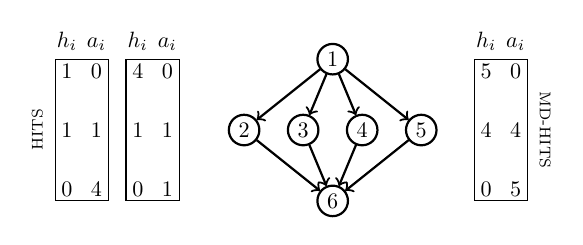
\begin{tikzpicture}[scale=.75]
\tikzset{every node/.style={scale=.8,thick,inner sep=2}}
    \node[circle,draw=black] (1) at (4,1.2) {1};
    \node[circle,draw=black] (2) at (2.5,0) {2};
    \node[circle,draw=black] (3) at (3.5,0) {3};
    \node[circle,draw=black] (4) at (4.5,0) {4};
    \node[circle,draw=black] (5) at (5.5,0) {5};
    \node[circle,draw=black] (6) at (4,-1.2) {6};
    \path[->,thick] (1) edge (2) (1) edge (3) (1) edge (4) (1) edge (5) (2) edge(6) (3) edge (6) (4) edge (6) (5) edge (6); 
    
    
    \node (hh) at (-.5,1.5) {$h_i$};
    \node (h1) at (-.5,1) {1};
    \node (h2) at (-.5, 0) {1};
    \node (h3) at (-.5,-1) {0};
    \node (aa) at (0,1.45) {$a_i$};
    \node (a1) at (0,1) {0};
    \node (a2) at (0, 0) {1};
    \node (a3) at (0,-1) {4};
    \draw (-.7,-1.2) rectangle (.2, 1.2);
    \node [rotate = 90] at (-1,0) {{\scriptsize HITS}};

    \node (hh) at (.7,1.5) {$h_i$};
    \node (h1) at (.7,1) {4};
    \node (h2) at (.7, 0) {1};
    \node (h3) at (.7,-1) {0};
    \node (aa) at (1.2,1.45) {$a_i$};
    \node (a1) at (1.2,1) {0};
    \node (a2) at (1.2, 0) {1};
    \node (a3) at (1.2,-1) {1};
    \draw (.5,-1.2) rectangle (1.4, 1.2);

    \node (hh) at (6.6,1.5) {$h_i$};
    \node (h1) at (6.6,1) {5};
    \node (h2) at (6.6, 0) {4};
    \node (h3) at (6.6,-1) {0};
    \node (aa) at (7.1,1.45) {$a_i$};
    \node (a1) at (7.1,1) {0};
    \node (a2) at (7.1, 0) {4};
    \node (a3) at (7.1,-1) {5};
    \draw (6.4,-1.2) rectangle (7.3, 1.2);
    \node [rotate = -90] at (7.6,0) {{\scriptsize MD-HITS}};
\end{tikzpicture}

\end{document}